\documentclass[12pt, a4paper]{article}

\usepackage{ctex}
\usepackage{float, booktabs, parskip}
\usepackage{amsmath, amsthm, amssymb, mathrsfs, bm}
\usepackage{graphicx, subfigure, svg}
\usepackage{hyperref, endnotes}

\setlength{\parindent}{4em}
\setlength{\parskip}{1em}
\allowdisplaybreaks[4]

\newcommand{\imat}{\bm}
\newcommand{\ivec}{\bm}
\newcommand{\tr}{{\rm tr}}
\newcommand{\diag}{{\rm diag}}
\newcommand{\softmax}{{\rm softmax}}
\newcommand{\sigmoid}{{\rm sig}}
\newcommand{\BN}{{\rm BN}}
\newcommand{\relu}{{\rm ReLU}}
\newcommand{\loss}{\mathcal{L}}

\newcommand{\thetam}{\imat{\Theta}}
\newcommand{\deltav}{\ivec{\delta}}
\newcommand{\av}{\ivec{a}}
\newcommand{\bv}{\ivec{b}}
\newcommand{\xv}{\ivec{x}}
\newcommand{\yv}{\ivec{y}}
\newcommand{\zv}{\ivec{z}}


\title{{\Huge{\textbf{Report on Homework 1 \\}}} —— Deep Learning}
\author{刘滨瑞 \\ 2021012579 \quad 未央-水木12}

\begin{document}

\maketitle

\section{Backpropogation}

    \stepcounter{subsection}

    \stepcounter{subsection}

    \subsection{Task Description}

    本节中的计算方法参考了Kaare Brandt Petersen和Michael Syskind Pedersen编著的《The Matrix Cookbook》。 \endnote{Petersen, K. B., Pedersen, M. S. The Matrix Cookbook. Technical University of Denmark, 2006}

    \subsubsection{Given a standard BatchNorm layer, please calculate the gradients of the output with respect to its parameters.}

        根据题述，$y_i = \BN_{\gamma, \beta}(x_i) = \gamma \hat{x_i} + \beta$。对$i \in \{1, 2, ..., m\}$，有：
        \begin{align}
        \frac{\partial{y_i}}{\partial{\gamma}} &= \hat{x_i} = \frac{x_i - \mu}{\sqrt{\sigma^2 + \epsilon}} \\
        \frac{\partial{y_i}}{\partial{\beta}} &= 1
        \end{align}

        其中$\mu_{\mathcal{B}} = \frac{1}{m} \sum_{i=1}^{m} x_i$，$\sigma_{\mathcal{B}} = \frac{1}{m} \sum_{i=1}^{m} (x_i - \mu_{\mathcal{B}})^2$.

    \subsubsection{Given a softmax function, please calculate the gradients of the output of a softmax function with respect to its input.}

        定义Softmax函数为：
        \begin{equation}\begin{aligned}
        \softmax(\xv) = \frac{\exp(\xv)}{\ivec{1}^T \exp(\xv)}
        \end{aligned}\end{equation}

        其中$\xv \in \mathbb{R}^n$，$\exp(\xv)$为逐元素函数，表示对$\xv$的每个元素求指数。若无特殊声明，其它函数在以向量作为输入时，同样视为逐元素函数。

        取Softmax函数的微分：
        \begin{align*}
        d (\softmax(\xv))
        &= d (\exp(\xv)) (\ivec{1}^T \exp(\xv))^{-1} + \exp(\xv) d ((\ivec{1}^T \exp(\xv))^{-1}) \\
        &= \frac{\exp(\xv) \otimes d \xv}{\ivec{1}^T \exp(\xv)} - \frac{\exp(\xv)}{(\ivec{1}^T \exp(\xv))^2} \otimes (\ivec{1}^T (\exp(\xv) \otimes d \xv)) \\
        &= \frac{\diag(\exp(\xv)) d \xv}{\ivec{1}^T \exp(\xv)} - \frac{\exp(\xv) \exp(\xv)^T d \xv}{(\ivec{1}^T \exp(\xv))^2} \\
        &= (\frac{\diag(\exp(\xv))}{\ivec{1}^T \exp(\xv)} - \frac{\exp(\xv) \exp(\xv)^T}{(\ivec{1}^T \exp(\xv))^2}) d \xv \\
        &= (\diag(\frac{\exp(\xv)}{\ivec{1}^T \exp(\xv)}) - \frac{\exp(\xv) \exp(\xv)^T}{(\ivec{1}^T \exp(\xv))^2})^T d \xv \\
        &= (\diag(\softmax(\xv)) - \softmax(\xv) \softmax(\xv)^T)^T d \xv
        \end{align*}

        因此，我们有：
        \begin{equation}\begin{aligned}
        \frac{\partial \softmax}{\partial \xv}
        &= \diag(\frac{\exp(\xv)}{\ivec{1}^T \exp(\xv)}) - \frac{\exp(\xv) \exp(\xv)^T}{(\ivec{1}^T \exp(\xv))^2} \\
        &= \diag(\softmax(\xv)) - \softmax(\xv) \softmax(\xv)^T
        \end{aligned}\end{equation}

    \subsubsection{Finish the detailed feed-forward computations of a batch of samples during a training iteration, coming with final predictions.}

        根据题意，我们设网络中的各个中间层的输出如下：
        \begin{align*}
        \zv_1 &= \thetam_1 \xv + \bv_1 \\
        \av_1 &= \sin(\zv_1) \\
        \av_{DP} &= \ivec{M} \otimes \av_1 \\
        \av_2 &= \thetam_2 \av_{DP} \\
        \zv_2 &= \av_2 + \bv_2 - \frac{1}{m} \sum_{i=1}^{m} \av_2^i\\
        \av_{BN} &= \relu(\zv_2) \\
        \av_3 &= \thetam_3 \av_{BN} + \bv_3 \\
        \zv_{ex1} &= \thetam_{ex1} \av_3 + \bv_{ex1} \\
        \av_{ex1} &= \relu(\zv_{ex1}) \\
        \zv_{ex2} &= \thetam_{ex2} \av_{ex1} + \bv_{ex2} \\
        \av_{ex2} &= \sigmoid(\zv_{ex2}) \\
        \zv_4 &= \thetam_4 (\av_{ex2} \otimes \av_3) + \bv_4 \\
        \hat{\yv} &= \softmax(\zv_4)
        \end{align*}

        其中$\relu(x) = \begin{cases}
                        x, &\text{if $x > 0$} \\
                        0, &\text{if $x \le 0$,}
                        \end{cases}$，
            $\sigmoid(x) = \frac{1}{1 + \exp(-x)}$。

        损失函数为：
        \begin{equation}\begin{aligned}
        \loss = -\frac{1}{m} \sum_{i=1}^{m} (\yv^{i})^{T} (\log{\hat{\yv^i}})
        \end{aligned}\end{equation}

    \subsubsection{Use the backpropagation algorithm we have learned in class and give the gradients of the overall loss in a mini-batch with respect to the parameters at each layer.}

        我们设$\loss = \frac{1}{m} \sum_{i=1}^{m} \loss^i$。其中：
        \begin{align*}
        \loss^i
        &= - (\yv^i)^{T} (\log{\hat{\yv^i}}) = - (\yv^i)^{T} \log{\softmax(\zv_4^i)} \\
        &= - (\yv^i)^{T} \zv_4^i + \log(\ivec{1}^T \exp(\zv_4^i))
        \end{align*}

        \begin{enumerate}

        \item 计算$\frac{\partial \loss^i}{\partial \thetam_4}$、$\frac{\partial \loss^i}{\partial \bv_4}$

            对$\loss^i$求微分，套用迹函数：
            \begin{align*}
            d \loss^i = \tr(d \loss^i)
            &= \tr(- (\yv^i)^{T} d \zv_4^i + \frac{\ivec{1}^T (\exp(\zv_4^i) \otimes d \zv_4^i)}{\ivec{1}^T \exp(\zv_4^i)}) \\
            &= \tr(- (\yv^i)^{T} d \zv_4^i + \frac{\exp(\zv_4^i)^T d \zv_4^i}{\ivec{1}^T \exp(\zv_4^i)}) \\
            &= \tr((\frac{\exp(\zv_4^i)^T}{\ivec{1}^T \exp(\zv_4^i)} - (\yv^i)^{T}) d \zv_4^i) \\
            &= \tr((\softmax(\zv_4^i) - \yv^i)^T d \zv_4^i)
            \end{align*}

            残差值为：
            \begin{equation}\begin{aligned}
            \deltav_4^i = \frac{\partial \loss^i}{\partial \zv_4^i} = \softmax(\zv_4^i) - \yv^i
            \end{aligned}\end{equation}

            继续对$d \zv_4^i$求微分:
            \begin{align*}
            d \zv_4^i
            &= d (\thetam_4 (\av_{ex2}^i \otimes \av_3^i) + \bv_4) \\
            &= d \thetam_4 (\av_{ex2}^i \otimes \av_3^i) + d \bv_4 + \thetam_4 (\av_3^i \otimes d \av_{ex2}^i + \av_{ex2}^i \otimes d \av_3^i)
            \end{align*}

            代入$d \loss^i$中：
            \begin{align*}
            d \loss^i &= \tr((\deltav_4^i)^T d \thetam_4 (\av_{ex2}^i \otimes \av_3^i)) + \tr((\deltav_4^i)^T d \bv_4) \\
                    &+ \tr((\deltav_4^i)^T \thetam_4 (\av_3^i \otimes d \av_{ex2}^i)) \\
                    &+ \tr((\deltav_4^i)^T \thetam_4 (\av_{ex2}^i \otimes d \av_3^i))
            \end{align*}
            我们简记上式中的后两项以此为$d l_{ex2}^i$和$d l_{3_{highway}}^i$。

            得到梯度:
            \begin{align*}
            \frac{\partial \loss^i}{\partial \thetam_4} &= \deltav_4^i (\av_{ex2}^i \otimes \av_3^i)^T \\
            \frac{\partial \loss^i}{\partial \bv_4} &= \deltav_4^i
            \end{align*}

            对$\loss^i$求和：
            \begin{align}
            \frac{\partial \loss}{\partial \thetam_4} &= \frac{1}{m} \sum_{i=1}^{m} \deltav_4^i (\av_{ex2}^i \otimes \av_3^i)^T \\
            \frac{\partial \loss}{\partial \bv_4} &= \frac{1}{m} \sum_{i=1}^{m} \deltav_4^i
            \end{align}

        \item 计算$\frac{\partial \loss^i}{\partial \thetam_{ex2}}$、$\frac{\partial \loss^i}{\partial \bv_{ex2}}$

            对$\av_{ex2}^i$求微分：
            \begin{align*}
            d \av_{ex2}^i
            &= d (\sigmoid(\zv_{ex2}^i)) \\
            &= (\sigmoid(\zv_{ex2}^i) \otimes (\ivec{1} - \sigmoid(\zv_{ex2}^i))) \otimes d \zv_{ex2}^i \\
            &= {\rm sigd}(\zv_{ex2}^i) \otimes d \zv_{ex2}^i
            \end{align*}
            其中${\rm sigd}(\zv_{ex2}^i) = \sigmoid(\zv_{ex2}^i) \otimes (\ivec{1} - \sigmoid(\zv_{ex2}^i))$。

            代入$d l_{ex2}^i$中：
            \begin{align*}
            d l_{ex2}^i
            &= \tr((\deltav_4^i)^T \thetam_4 (\av_3^i \otimes d \av_{ex2}^i)) \\
            &= \tr\{(\deltav_4^i)^T \thetam_4 [\av_3^i \otimes ({\rm sigd}(\zv_{ex2}^i) \otimes d \zv_{ex2}^i)]\} \\
            &= \tr\{(\deltav_4^i)^T \thetam_4 [(\av_3^i \otimes {\rm sigd}(\zv_{ex2}^i)) \otimes d \zv_{ex2}^i]\} \\
            &= \tr\{[(\thetam_4^T \deltav_4^i) \otimes (\av_3^i \otimes {\rm sigd}(\zv_{ex2}^i))]^T d \zv_{ex2}^i\}
            \end{align*}

            残差值为：
            \begin{equation}\begin{aligned}
            \deltav_{ex2}^i = \frac{\partial \loss^i}{\partial \zv_{ex2}^i}
            &= \frac{\partial \loss^i}{\partial l_{ex2}^i} \frac{\partial l_{ex2}^i}{\partial \zv_{ex2}^i} \\
            &= (\thetam_4^T \deltav_4^i) \otimes (\av_3^i \otimes {\rm sigd}(\zv_{ex2}^i)) \\
            &= (\thetam_4^T \deltav_4^i) \otimes \av_3^i \otimes \sigmoid(\zv_{ex2}^i) \otimes (\ivec{1} - \sigmoid(\zv_{ex2}^i))
            \end{aligned}\end{equation}

            继续对$d \zv_{ex2}^i$求微分:
            \begin{align*}
            d \zv_{ex2}^i
            &= d (\thetam_{ex2} \av_{ex1}^i + \bv_{ex2}) \\
            &= d \thetam_{ex2} \av_{ex1}^i + d \bv_{ex2} + \thetam_{ex2} d \av_{ex1}^i
            \end{align*}

            代入$d l_{ex2}^i$中：
            \begin{align*}
            d l_{ex2}^i &= \tr((\deltav_{ex2}^i)^T d \thetam_{ex2} \av_{ex1}^i) \\
                        &+ \tr((\deltav_{ex2}^i)^T d \bv_{ex2}) \\
                        &+ \tr((\deltav_{ex2}^i)^T \thetam_{ex2} d \av_{ex1}^i)
            \end{align*}
            我们简记$d l_{ex1}^i = \tr((\deltav_{ex2}^i)^T \thetam_{ex2} d \av_{ex1}^i)$。

            得到梯度:
            \begin{align*}
            \frac{\partial \loss^i}{\partial \thetam_{ex2}} &= \deltav_{ex2}^i (\av_{ex1}^i)^T \\
            \frac{\partial \loss^i}{\partial \bv_{ex2}} &= \deltav_{ex2}^i
            \end{align*}

            对$\loss^i$求和：
            \begin{align}
            \frac{\partial \loss}{\partial \thetam_{ex2}} &= \frac{1}{m} \sum_{i=1}^{m} \deltav_{ex2}^i (\av_{ex1}^i)^T \\
            \frac{\partial \loss}{\partial \bv_{ex2}} &= \frac{1}{m} \sum_{i=1}^{m} \deltav_{ex2}^i
            \end{align}

        \item 计算$\frac{\partial \loss^i}{\partial \thetam_{ex1}}$、$\frac{\partial \loss^i}{\partial \bv_{ex1}}$

            对$\av_{ex1}^i$求微分：
            \begin{align*}
            d \av_{ex1}^i = d \relu(\zv_{ex1}) = \relu^{\prime}(\zv_{ex1}^i) \otimes d \zv_{ex1}^i
            \end{align*}
            其中$\relu^{\prime}(x) =
                                    \begin{cases}
                                    1, &\text{if $x > 0$} \\
                                    0, &\text{if $x \le 0$,}
                                    \end{cases}$，是逐元素函数。

            代入$d l_{ex1}^i$中：
            \begin{align*}
            d l_{ex1}^i
            &= \tr((\deltav_{ex2}^i)^T \thetam_{ex2} d \av_{ex1}^i) \\
            &= \tr\{(\deltav_{ex2}^i)^T \thetam_{ex2} [\relu^{\prime}(\zv_{ex1}^i) \otimes d \zv_{ex1}^i]\} \\
            &= \tr\{[(\thetam_{ex2}^T \deltav_{ex2}^i) \otimes \relu^{\prime}(\zv_{ex1}^i)]^T d \zv_{ex1}^i\}
            \end{align*}

            残差值为：
            \begin{equation}\begin{aligned}
            \deltav_{ex1}^i = \frac{\partial \loss^i}{\partial \zv_{ex1}^i}
            &= \frac{\partial \loss^i}{\partial l_{ex1}^i} \frac{\partial l_{ex1}^i}{\partial \zv_{ex1}^i} \\
            &= (\thetam_{ex2}^T \deltav_{ex2}^i) \otimes \relu^{\prime}(\zv_{ex1}^i)
            \end{aligned}\end{equation}

            继续对$d \zv_{ex1}^i$求微分:
            \begin{align*}
            d \zv_{ex1}^i
            &= d (\thetam_{ex1} \av_3^i + \bv_{ex1}) \\
            &= d \thetam_{ex1} \av_3^i + d \bv_{ex1} + \thetam_{ex1} d \av_3^i
            \end{align*}

            代入$d l_{ex1}^i$中：
            \begin{align*}
            d l_{ex1}^i &= \tr((\deltav_{ex1}^i)^T d \thetam_{ex1} \av_3^i) \\
                        &+ \tr((\deltav_{ex1}^i)^T d \bv_{ex1}) \\
                        &+ \tr((\deltav_{ex1}^i)^T \thetam_{ex1} d \av_3^i)
            \end{align*}

            我们简记$d l_{3_{normal}}^i = \tr((\deltav_{ex1}^i)^T \thetam_{ex1} d \av_3^i)$。有：
            \begin{align*}
            d l_3^i
            &= d l_{3_{normal}}^i + d l_{3_{highway}}^i \\
            &= \tr((\deltav_{ex1}^i)^T \thetam_{ex1} d \av_3^i) + \tr((\deltav_4^i)^T \thetam_4 (\av_{ex2}^i \otimes d \av_3^i)) \\
            &= \tr((\thetam_{ex1}^T \deltav_{ex1}^i)^T d \av_3^i) + \tr(((\thetam_4^T \deltav_4^i) \otimes \av_{ex2}^i)^T d \av_3^i) \\
            &= \tr((\thetam_{ex1}^T \deltav_{ex1}^i + (\thetam_4^T \deltav_4^i) \otimes \av_{ex2}^i)^T d \av_3^i)
            \end{align*}

            得到梯度:
            \begin{align*}
            \frac{\partial \loss^i}{\partial \thetam_{ex1}} &= \deltav_{ex1}^i (\av_3^i)^T \\
            \frac{\partial \loss^i}{\partial \bv_{ex1}} &= \deltav_{ex1}^i
            \end{align*}

            对$\loss^i$求和：
            \begin{align}
            \frac{\partial \loss}{\partial \thetam_{ex1}} &= \frac{1}{m} \sum_{i=1}^{m} \deltav_{ex1}^i (\av_3^i)^T \\
            \frac{\partial \loss}{\partial \bv_{ex1}} &= \frac{1}{m} \sum_{i=1}^{m} \deltav_{ex1}^i
            \end{align}

        \item 计算$\frac{\partial \loss^i}{\partial \thetam_3}$、$\frac{\partial \loss^i}{\partial \bv_3}$

            考虑$d l_3^i$：
            \begin{align*}
            d l_3^i = \tr((\thetam_{ex1}^T \deltav_{ex1}^i + (\thetam_4^T \deltav_4^i) \otimes \av_{ex2}^i)^T d \av_3^i)
            \end{align*}

            残差值为：
            \begin{equation}\begin{aligned}
            \deltav_3^i = \frac{\partial \loss^i}{\partial \zv_3^i} = \frac{\partial \loss^i}{\partial \av_3^i}
            &= \frac{\partial \loss^i}{\partial l_3^i} \frac{\partial l_3^i}{\partial \av_3^i} \\
            &= \thetam_{ex1}^T \deltav_{ex1}^i + (\thetam_4^T \deltav_4^i) \otimes \av_{ex2}^i
            \end{aligned}\end{equation}
            其中我们指定：$\zv_3^i = \av_3^i$。

            继续对$\av_3^i$求微分：
            \begin{align*}
            d \av_3^i
            &= d (\thetam_3 \av_{BN}^i + \bv_3) \\
            &= d \thetam_3 \av_{BN}^i + d \bv_3 + \thetam_3 d \av_{BN}^i
            \end{align*}

            代入$d l_3^i$中：
            \begin{align*}
            d l_3^i &= \tr((\deltav_3^i)^T d \thetam_3 \av_{BN}^i) \\
                        &+ \tr((\deltav_3^i)^T d \bv_3) \\
                        &+ \tr((\deltav_3^i)^T \thetam_3 d \av_{BN}^i)
            \end{align*}
            我们简记$d l_{BN}^i = \tr((\deltav_3^i)^T \thetam_3 d \av_{BN}^i)$。

            得到梯度:
            \begin{align*}
            \frac{\partial \loss^i}{\partial \thetam_3} &= \deltav_3^i (\av_{BN}^i)^T \\
            \frac{\partial \loss^i}{\partial \bv_3} &= \deltav_3^i
            \end{align*}

            对$\loss^i$求和：
            \begin{align}
            \frac{\partial \loss}{\partial \thetam_3} &= \frac{1}{m} \sum_{i=1}^{m} \deltav_3^i (\av_{BN}^i)^T \\
            \frac{\partial \loss}{\partial \bv_3} &= \frac{1}{m} \sum_{i=1}^{m} \deltav_3^i
            \end{align}

        \item 计算$\frac{\partial \loss^i}{\partial \thetam_2}$、$\frac{\partial \loss^i}{\partial \bv_2}$

            对$\av_{BN}^i$求微分：
            \begin{align*}
            d \av_{BN}^i = d \relu(\zv_2) = \relu^{\prime}(\zv_2^i) \otimes d \zv_2^i
            \end{align*}

            代入$d l_{BN}^i$中：
            \begin{align*}
            d l_{BN}^i
            &= \tr((\deltav_3^i)^T \thetam_3 d \av_{BN}^i) \\
            &= \tr\{(\deltav_3^i)^T \thetam_3 [\relu^{\prime}(\zv_2^i) \otimes d \zv_2^i]\} \\
            &= \tr\{[(\thetam_3^T \deltav_3^i) \otimes \relu^{\prime}(\zv_2^i)]^T d \zv_2^i\}
            \end{align*}

            残差值为：
            \begin{equation}\begin{aligned}
            \deltav_2^i = \frac{\partial \loss^i}{\partial \zv_2^i}
            &= \frac{\partial \loss^i}{\partial l_{BN}^i} \frac{\partial l_{BN}^i}{\partial \zv_2^i} \\
            &= (\thetam_3^T \deltav_3^i) \otimes \relu^{\prime}(\zv_2^i)
            \end{aligned}\end{equation}

            继续对$d \zv_2^i$求微分:
            \begin{align*}
            d \zv_2^i
            &= d (\av_2^i + \bv_2 - \frac{1}{m} \sum_{j=1}^{m} \av_2^j) \\
            &= d (\thetam_2 \av_{DP}^i + \bv_2 - \frac{1}{m} \sum_{j=1}^{m} \thetam_2 \av_{DP}^j) \\
            &= d \thetam_2 \av_{DP}^i + d \bv_2 + \thetam_2 d \av_{DP}^i - \frac{1}{m} (d \thetam_2 \sum_{j=1}^{m} \av_{DP}^j + \sum_{j=1}^{m} \thetam_2 d \av_{DP}^j) \\
            &= d \thetam_2 (\av_{DP}^i - \frac{1}{m} \sum_{j=1}^{m} \av_{DP}^j) + d \bv_2 + \thetam_2 (d \av_{DP}^i - \frac{1}{m} \sum_{j=1}^{m} d \av_{DP}^j)
            \end{align*}

            代入$d l_{BN}^i$中：
            \begin{align*}
            d l_{BN}^i &= \tr((\deltav_2^i)^T d \thetam_2 (\av_{DP}^i - \frac{1}{m} \sum_{j=1}^{m} \av_{DP}^j)) \\
                        &+ \tr((\deltav_2^i)^T d \bv_2) \\
                        &+ \tr((\deltav_2^i)^T \thetam_2 (d \av_{DP}^i - \frac{1}{m} \sum_{j=1}^{m} d \av_{DP}^j))
            \end{align*}

            对$l_{BN}^i$求和：
            \begin{align*}
            d l_{BN} = &\tr((\frac{1}{m} \sum_{i = 1}^{m} \deltav_2^i (\av_{DP}^i - \frac{1}{m} \sum_{j=1}^{m} \av_{DP}^j)^T)^T d \thetam_2) \\
                        &+ \tr((\frac{1}{m} \sum_{i = 1}^{m} \deltav_2^i)^T d \bv_2) \\
                        &+ \tr((\frac{1}{m} \sum_{i = 1}^{m} \deltav_2^i (d \av_{DP}^i - \frac{1}{m} \sum_{j=1}^{m} d \av_{DP}^j)^T)^T \thetam_2)
            \end{align*}
            我们简记：
            \begin{align*}
            d l_{DP}
            &= \tr((\frac{1}{m} \sum_{i = 1}^{m} \deltav_2^i (d \av_{DP}^i - \frac{1}{m} \sum_{j=1}^{m} d \av_{DP}^j)^T)^T \thetam_2) \\
            &= \tr((\frac{1}{m} \sum_{i = 1}^{m} (\deltav_2^i - \frac{1}{m} \sum_{j = 1}^{m} \deltav_2^j) (d \av_{DP}^i)^T)^T \thetam_2)
            \end{align*}
            对$i \in \{1, 2, ..., m\}$，定义：
            \begin{align*}
            d l_{DP}^i
            &= \tr(((\deltav_2^i - \frac{1}{m} \sum_{j = 1}^{m} \deltav_2^j) (d \av_{DP}^i)^T)^T \thetam_2) \\
            &= \tr((\deltav_2^i - \frac{1}{m} \sum_{j = 1}^{m} \deltav_2^j)^T \thetam_2 d \av_{DP}^i)
            \end{align*}
            满足：$d l_{DP} = \frac{1}{m} \sum_{i = 1}^{m} d l_{DP}^i$。

            关于$\loss$的梯度为：
            \begin{align}
            \frac{\partial \loss}{\partial \thetam_2} &= \frac{1}{m} \sum_{i = 1}^{m} \deltav_2^i (\av_{DP}^i - \frac{1}{m} \sum_{j=1}^{m} \av_{DP}^j)^T \\
            \frac{\partial \loss}{\partial \bv_2} &= \frac{1}{m} \sum_{i = 1}^{m} \deltav_2^i
            \end{align}

        \item 计算$\frac{\partial \loss^i}{\partial \thetam_1}$、$\frac{\partial \loss^i}{\partial \bv_1}$

            对$\av_{DP}^i$求微分：
            \begin{align*}
            d \av_{DP}^i = d (\ivec{M} \otimes \sin(\zv_1^i))
            &= \ivec{M} \otimes d \sin(\zv_1^i) \\
            &= \ivec{M} \otimes \cos(\zv_1^i) \otimes d \zv_1^i
            \end{align*}

            代入$d l_{DP}^i$中：
            \begin{align*}
            d l_{DP}^i
            &= \tr((\deltav_2^i - \frac{1}{m} \sum_{j = 1}^{m} \deltav_2^j)^T \thetam_2 d \av_{DP}^i) \\
            &= \tr\{[\thetam_2^T (\deltav_2^i - \frac{1}{m} \sum_{j = 1}^{m} \deltav_2^j)]^T [(\ivec{M} \otimes \cos(\zv_1^i)) \otimes d \zv_1^i]\} \\
            &= \tr\{[(\thetam_2^T (\deltav_2^i - \frac{1}{m} \sum_{j = 1}^{m} \deltav_2^j)) \otimes (\ivec{M} \otimes \cos(\zv_1^i))]^T d \zv_1^i\} \\
            \end{align*}

            残差值为：
            \begin{equation}\begin{aligned}
            \deltav_1^i = \frac{\partial \loss^i}{\partial \zv_1^i}
            &= \frac{\partial \loss^i}{\partial l_{DP}^i} \frac{\partial l_{DP}^i}{\partial \zv_1^i} \\
            &= (\thetam_2^T (\deltav_2^i - \frac{1}{m} \sum_{j = 1}^{m} \deltav_2^j)) \otimes (\ivec{M} \otimes \cos(\zv_1^i))
            \end{aligned}\end{equation}

            继续对$d \zv_1^i$求微分:
            \begin{align*}
            d \zv_1^i
            &= d (\thetam_1 \xv^i + \bv_1) \\
            &= d \thetam_1 \xv^i + d \bv_1
            \end{align*}

            代入$d l_{DP}^i$中：
            \begin{align*}
            d l_{DP}^i = \tr((\deltav_1^i)^T d \thetam_1 \xv^i) + \tr((\deltav_1^i)^T d \bv_1)
            \end{align*}

            得到梯度:
            \begin{align*}
            \frac{\partial \loss^i}{\partial \thetam_1} &= \deltav_1^i (\xv^i)^T \\
            \frac{\partial \loss^i}{\partial \bv_1} &= \deltav_1^i
            \end{align*}

            对$\loss^i$求和：
            \begin{align}
            \frac{\partial \loss}{\partial \thetam_1} &= \frac{1}{m} \sum_{i=1}^{m} \deltav_1^i (\xv^i)^T \\
            \frac{\partial \loss}{\partial \bv_1} &= \frac{1}{m} \sum_{i=1}^{m} \deltav_1^i
            \end{align}

        \end{enumerate}

        综上，反向传播过程中优化目标函数对各参数的梯度为：
        \begin{align*}
        \frac{\partial \loss}{\partial \thetam_4} &= \frac{1}{m} \sum_{i=1}^{m} \deltav_4^i (\av_{ex2}^i \otimes \av_3^i)^T \\
        \frac{\partial \loss}{\partial \bv_4} &= \frac{1}{m} \sum_{i=1}^{m} \deltav_4^i \\
        \frac{\partial \loss}{\partial \thetam_{ex2}} &= \frac{1}{m} \sum_{i=1}^{m} \deltav_{ex2}^i (\av_{ex1}^i)^T \\
        \frac{\partial \loss}{\partial \bv_{ex2}} &= \frac{1}{m} \sum_{i=1}^{m} \deltav_{ex2}^i \\
        \frac{\partial \loss}{\partial \thetam_{ex1}} &= \frac{1}{m} \sum_{i=1}^{m} \deltav_{ex1}^i (\av_3^i)^T \\
        \frac{\partial \loss}{\partial \bv_{ex1}} &= \frac{1}{m} \sum_{i=1}^{m} \deltav_{ex1}^i \\
        \frac{\partial \loss}{\partial \thetam_3} &= \frac{1}{m} \sum_{i=1}^{m} \deltav_3^i (\av_{BN}^i)^T \\
        \frac{\partial \loss}{\partial \bv_3} &= \frac{1}{m} \sum_{i=1}^{m} \deltav_3^i \\
        \frac{\partial \loss}{\partial \thetam_2} &= \frac{1}{m} \sum_{i = 1}^{m} \deltav_2^i (\av_{DP}^i - \frac{1}{m} \sum_{j=1}^{m} \av_{DP}^j)^T \\
        \frac{\partial \loss}{\partial \bv_2} &= \frac{1}{m} \sum_{i = 1}^{m} \deltav_2^i \\
        \frac{\partial \loss}{\partial \thetam_1} &= \frac{1}{m} \sum_{i=1}^{m} \deltav_1^i (\xv^i)^T \\
        \frac{\partial \loss}{\partial \bv_1} &= \frac{1}{m} \sum_{i=1}^{m} \deltav_1^i
        \end{align*}
        其中：
        \begin{align*}
        \deltav_4^i = \frac{\partial \loss^i}{\partial \zv_4^i} &= \softmax(\zv_4^i) - \yv^i \\
        \deltav_{ex2}^i = \frac{\partial \loss^i}{\partial \zv_{ex2}^i} &= (\thetam_4^T \deltav_4^i) \otimes \av_3^i \otimes \sigmoid(\zv_{ex2}^i) \otimes (\ivec{1} - \sigmoid(\zv_{ex2}^i)) \\
        \deltav_{ex1}^i = \frac{\partial \loss^i}{\partial \zv_{ex1}^i} &= (\thetam_{ex2}^T \deltav_{ex2}^i) \otimes \relu^{\prime}(\zv_{ex1}^i) \\
        \deltav_3^i = \frac{\partial \loss^i}{\partial \zv_3^i} &= \thetam_{ex1}^T \deltav_{ex1}^i + (\thetam_4^T \deltav_4^i) \otimes \av_{ex2}^i \\
        \deltav_2^i = \frac{\partial \loss^i}{\partial \zv_2^i} &= (\thetam_3^T \deltav_3^i) \otimes \relu^{\prime}(\zv_2^i) \\
        \deltav_1^i = \frac{\partial \loss^i}{\partial \zv_1^i} &= (\thetam_2^T (\deltav_2^i - \frac{1}{m} \sum_{j = 1}^{m} \deltav_2^j)) \otimes (\ivec{M} \otimes \cos(\zv_1^i))
        \end{align*}

\section{Multilayer Perceptron}

    \stepcounter{subsection}

    \stepcounter{subsection}

    \stepcounter{subsection}

    \stepcounter{subsection}

    \subsection{Task Description}

    运行环境为：Windows 10 22H2，Python 3.9.18，PyTorch 1.12.1。

    \subsubsection{Implement forward propagation and backward propagation algorithms. Train the network, plot the change in loss during training, and showcase some predictions from your models.}

        前向传播算法和反向传播算法已在代码中实现，参见./MLP/model.py中注释含有“TODO”的部分。

        值得一提的是，考虑到本题中的MLP模型使用ReLU函数作为激活函数，因此我们在初始化参数时使用了\textbf{He Initialization}方法。 \endnote{He, K., Zhang, X., Ren, S., Sun, J. Delving deep into rectifiers: surpassing human-level performance on imagenet classification. IEEE Computer Society, 2015}

        将训练完成的模型在测试集上进行测试，\textbf{均方误差为0.6138}，\textbf{平均绝对误差为0.5460}。

        在训练过程中，损失函数的变化曲线如图1所示。由于我们取每个batch的计算为一个iteration，因此图1中存在着一定的震荡现象。
        即便如此，我们仍然可以观察到在1k次迭代后，损失函数已经大致收敛。

        \begin{figure}[htbp]
        \centering
        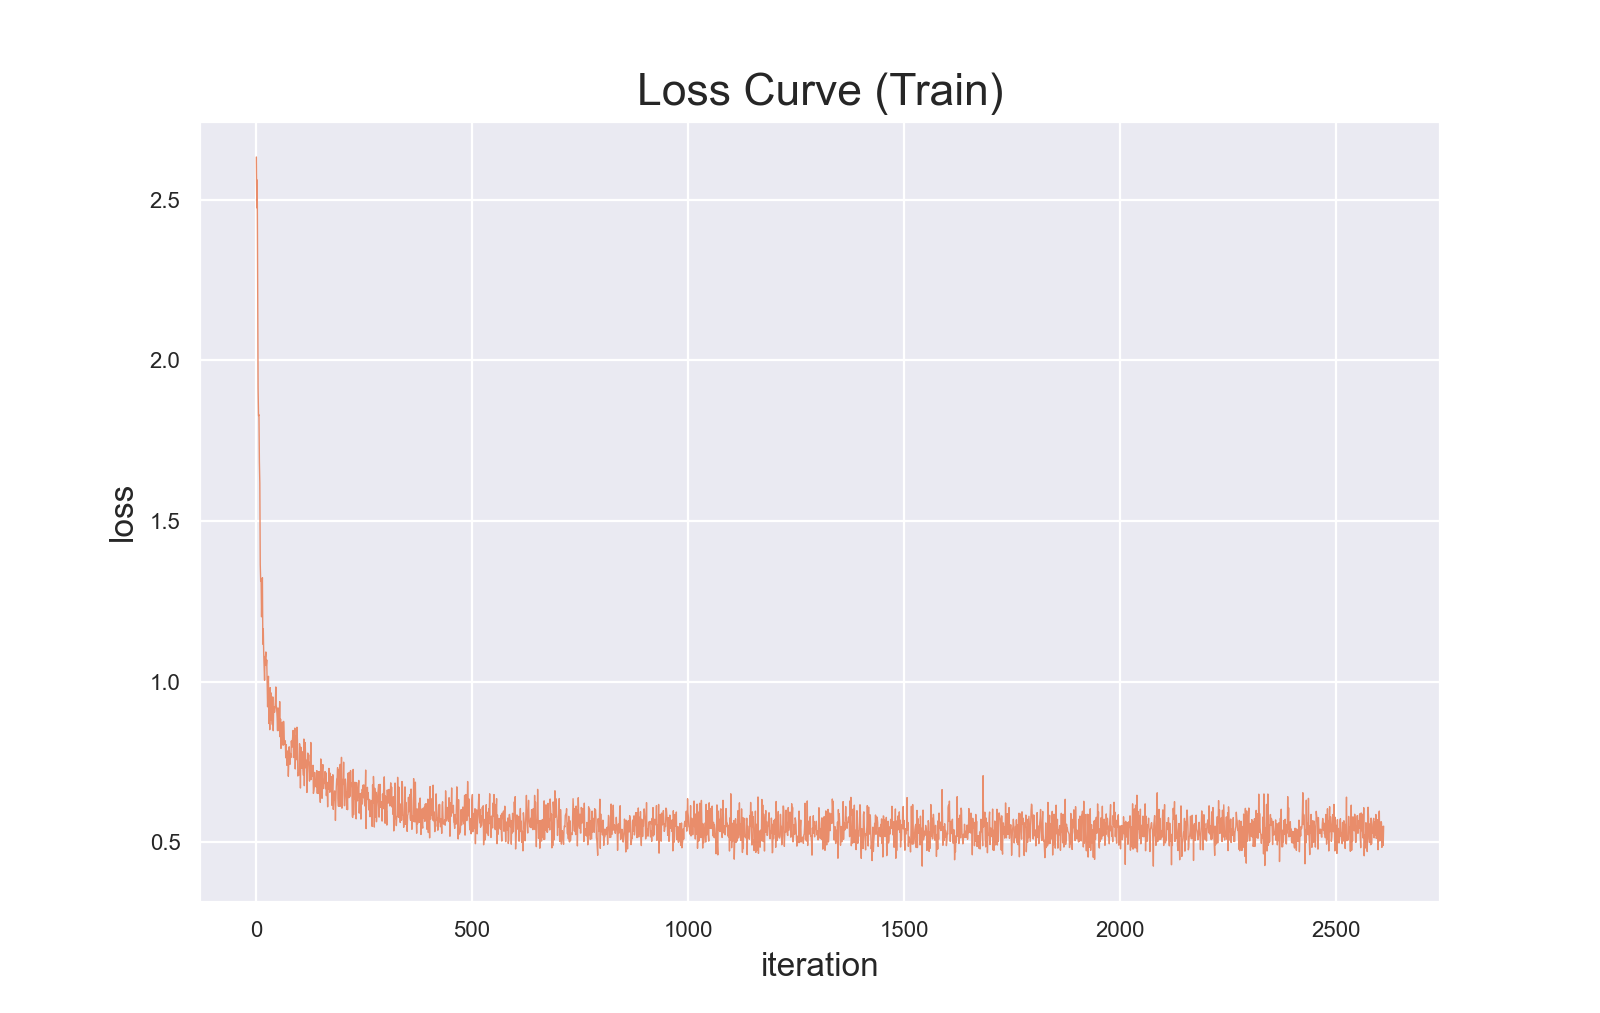
\includegraphics[width=0.72\textwidth]{./assets/MLP_loss_curve_train.png}
        \caption{训练集上的损失函数的变化曲线}
        \end{figure}

        我们在每个epoch后在验证集上测试模型的误差，以检查模型的过拟合情况。在验证集下，损失函数的变化曲线如图2所示。
        可以看出，模型在验证集上的误差并未随着epoch的增加而提高，这说明代码中的早停机制发挥了作用，同时也意味着我们训练所得的模型过拟合程度较低。

        \begin{figure}[htbp]
        \centering
        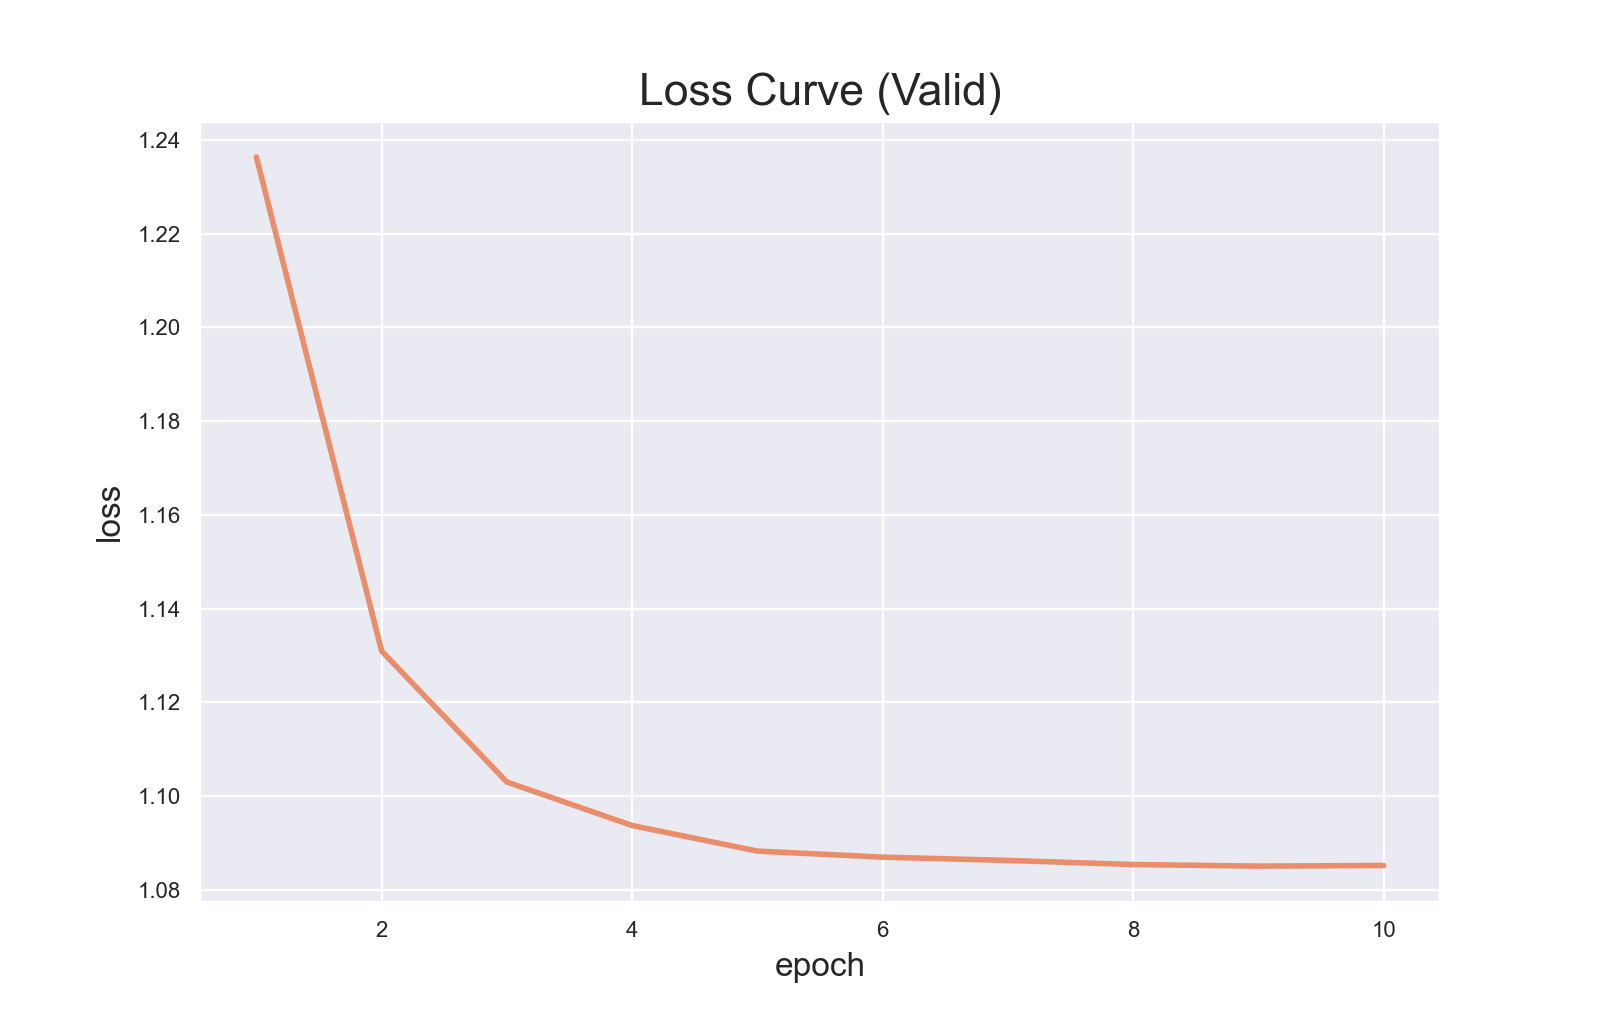
\includegraphics[width=0.72\textwidth]{./assets/MLP_loss_curve_valid.png}
        \caption{验证集上的损失函数的变化曲线}
        \end{figure}

        \begin{figure}[htbp]
        \centering
        \subfigure[Time id: 400]{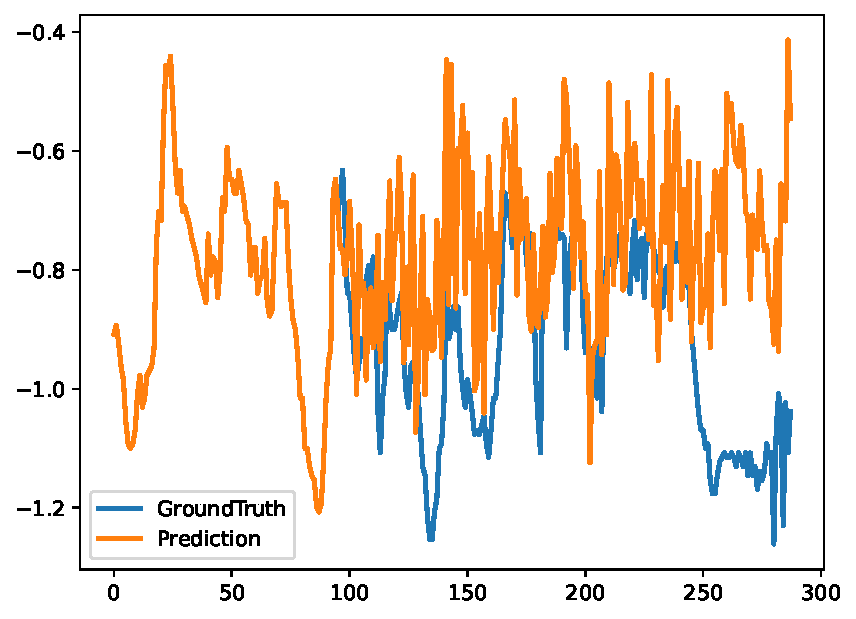
\includegraphics[width=0.36\textwidth]{./assets/MLP_400.pdf}}
        \subfigure[Ttime id: 700]{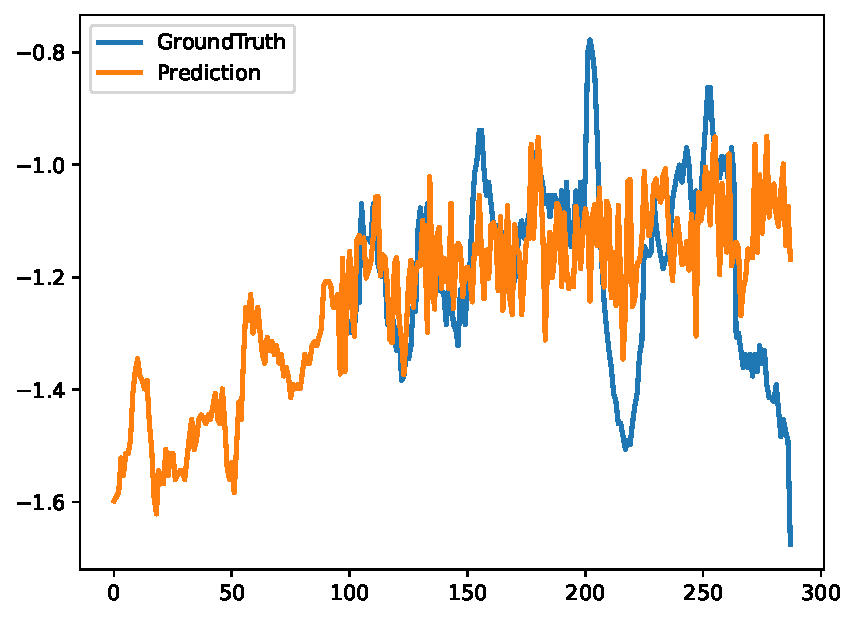
\includegraphics[width=0.36\textwidth]{./assets/MLP_700.pdf}}
        \quad
        \subfigure[Time id: 1000]{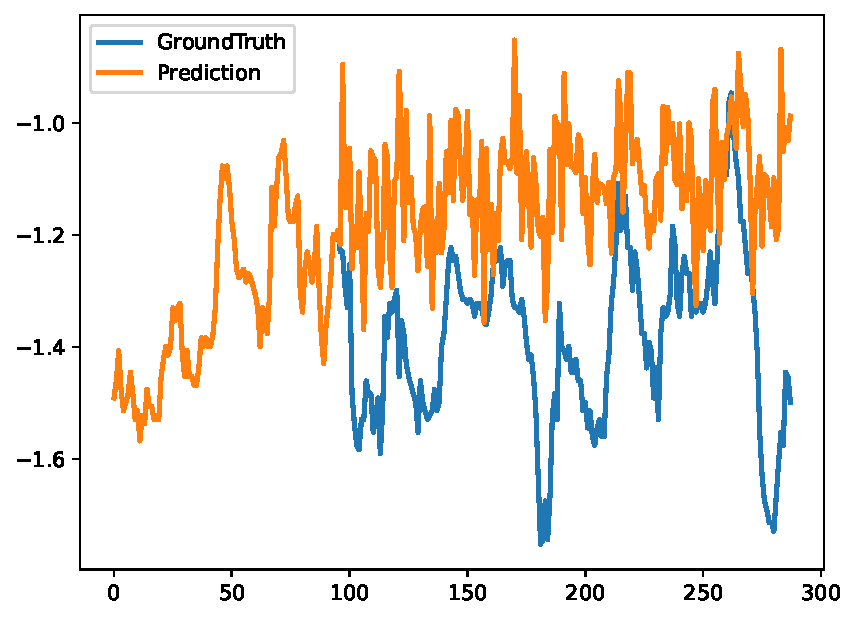
\includegraphics[width=0.36\textwidth]{./assets/MLP_1000.pdf}}
        \subfigure[Time id: 1300]{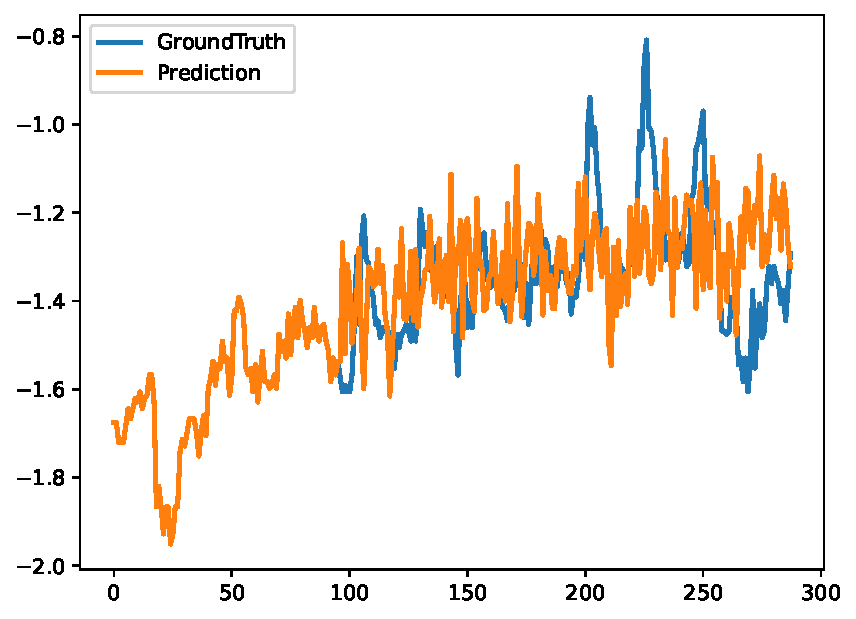
\includegraphics[width=0.36\textwidth]{./assets/MLP_1300.pdf}}
        \quad
        \subfigure[Time id: 1600]{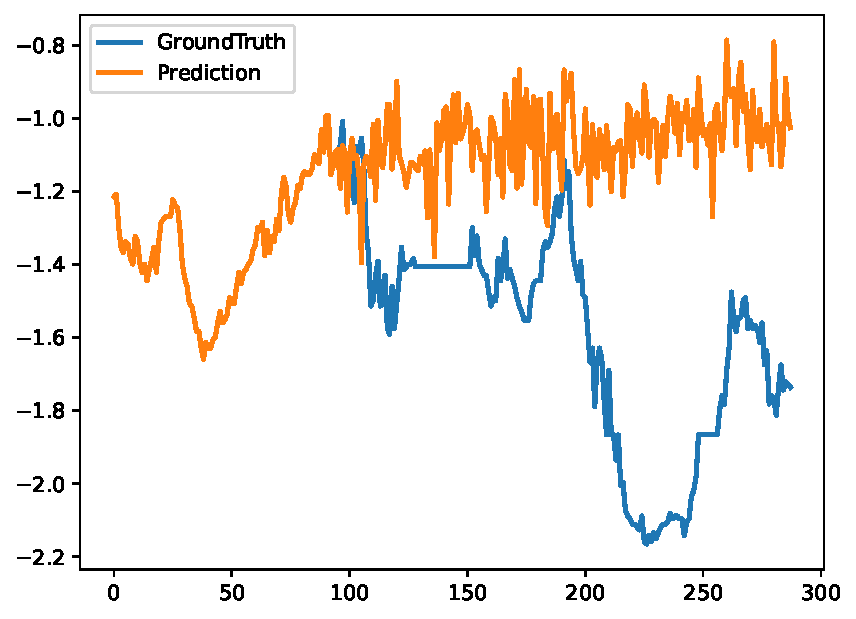
\includegraphics[width=0.36\textwidth]{./assets/MLP_1600.pdf}}
        \subfigure[Ttime id: 1900]{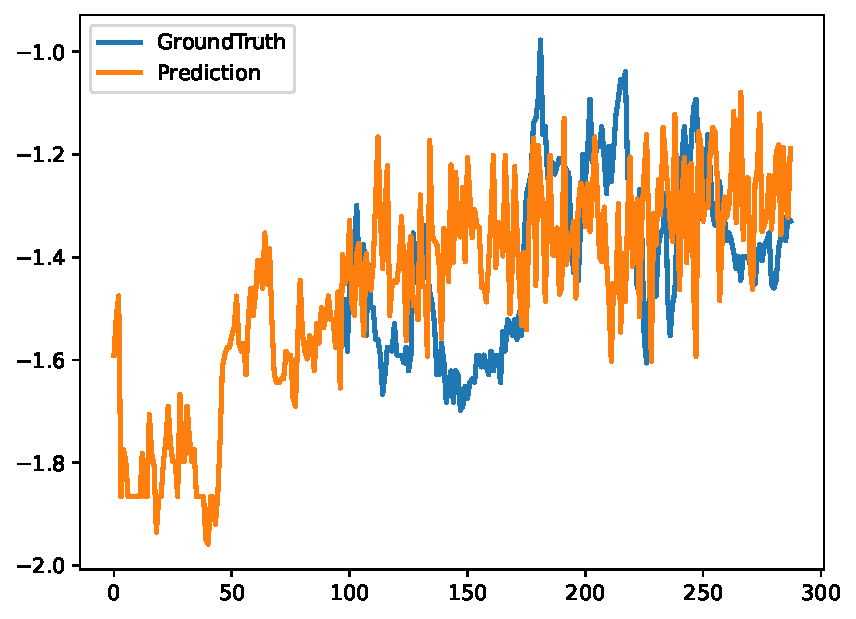
\includegraphics[width=0.36\textwidth]{./assets/MLP_1900.pdf}}
        \quad
        \subfigure[Time id: 2200]{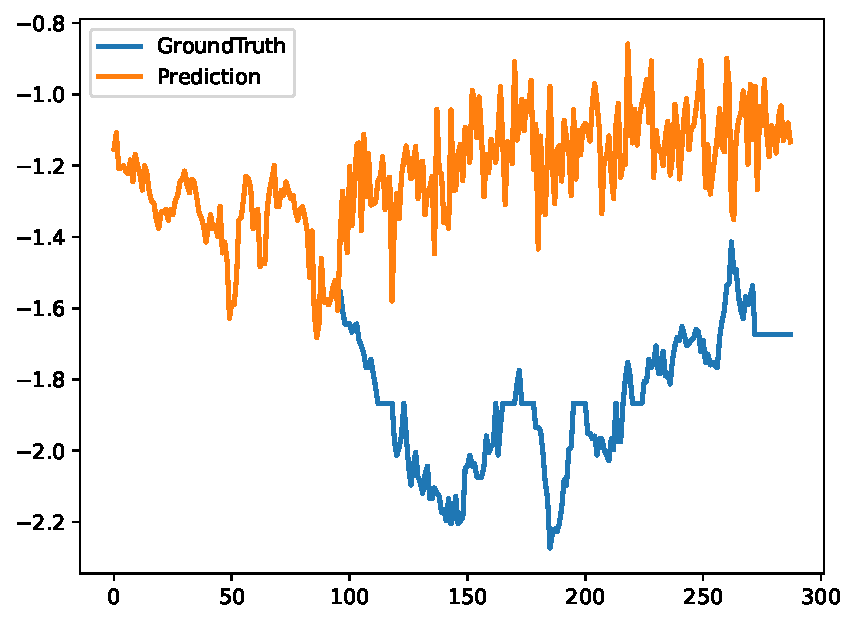
\includegraphics[width=0.36\textwidth]{./assets/MLP_2200.pdf}}
        \subfigure[Time id: 2500]{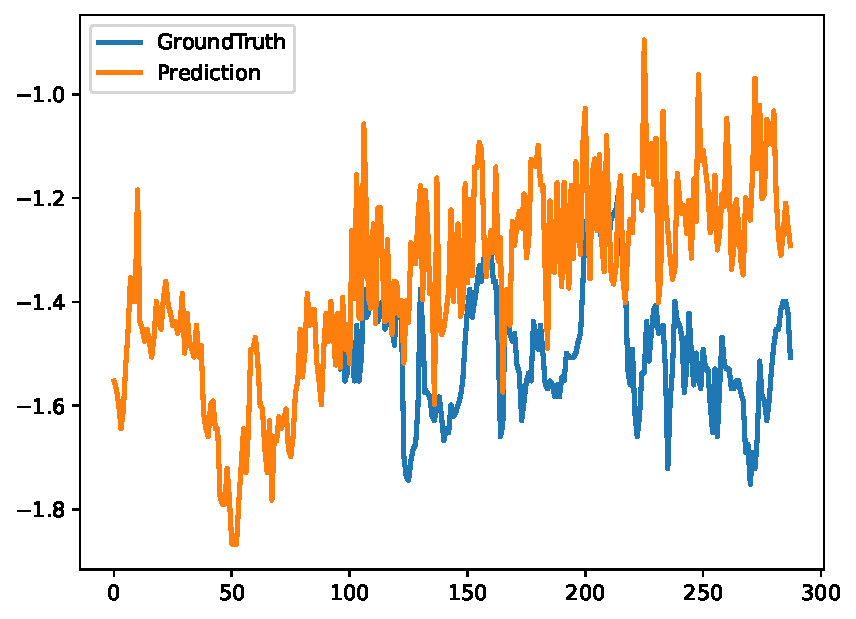
\includegraphics[width=0.36\textwidth]{./assets/MLP_2500.pdf}}
        \caption{模型在测试集上的预测结果}
        \end{figure}

        如图3所示，我们将模型在测试集上的预测结果绘制为图像，与真实值相对比。我们发现，模型的预测效果并不是特别理想。
        在原始数据较为平滑的时段（如Time id为700、1300、1900时），模型给出的预测值尚且较为贴近真实值，
        但是在原始数据波动较大的时段（如Time id为1600、2200时），模型并没有成功建模数据所发生的剧烈变化。
        我们推测，原因可能是模型参数量较小，拟合能力不足；也可能是因为MLP模型并不擅长处理长时段下的时序预测问题。

    \subsubsection{Train the network using proper hyper-parameters (batch size, learning rate, etc) and report the test MSE, which should not exceed 0.6.}

        我们认为，学习率过高会导致优化过程不稳定，而学习率过低则会导致收敛速度降低。
        而batch\_size的增大则会使得模型更多地受到数据噪声的影响，从而导致模型的效果降低。

        调整学习率（learning\_rate）和batch\_size，模型在测试集上的均方误差和平均绝对误差测试结果如图4、图5所示。

        \begin{figure}[htbp]
        \centering
        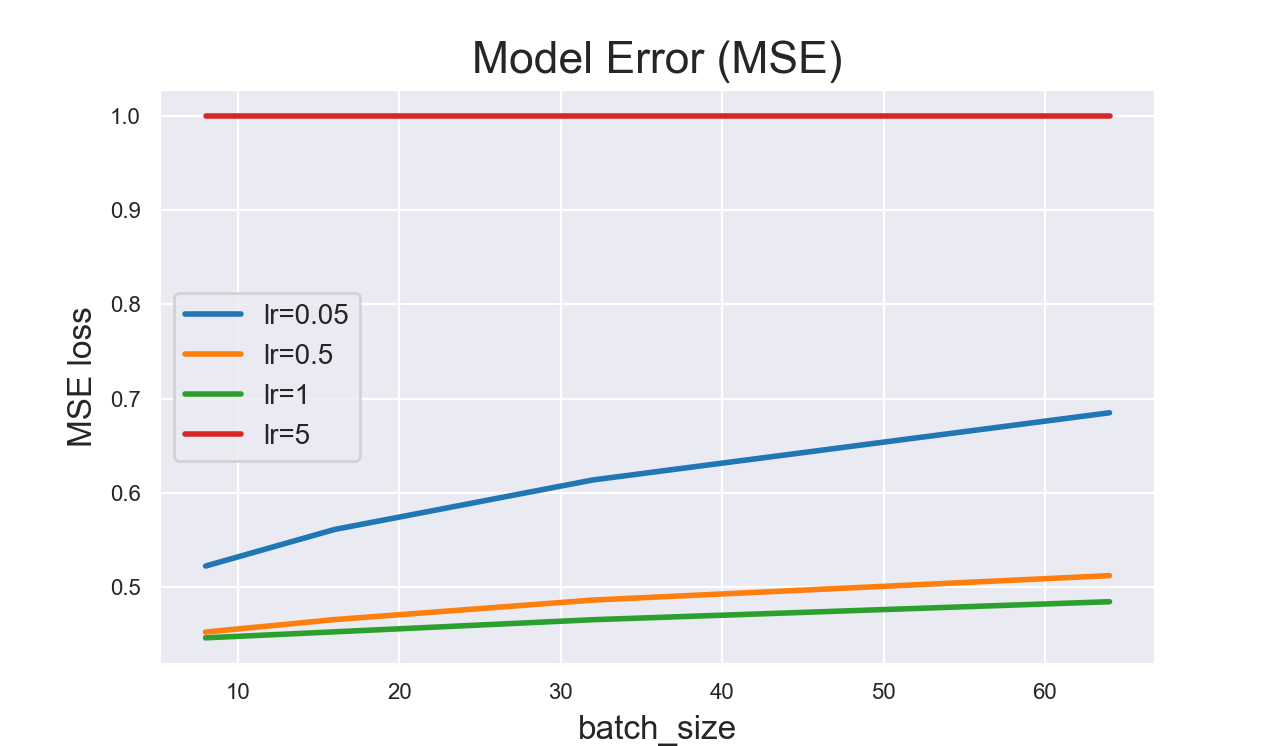
\includegraphics[width=0.90\textwidth]{./assets/MLP_MSE.png}
        \caption{不同超参数下，模型在测试集上的均方误差}
        \end{figure}

        \begin{figure}[htbp]
        \centering
        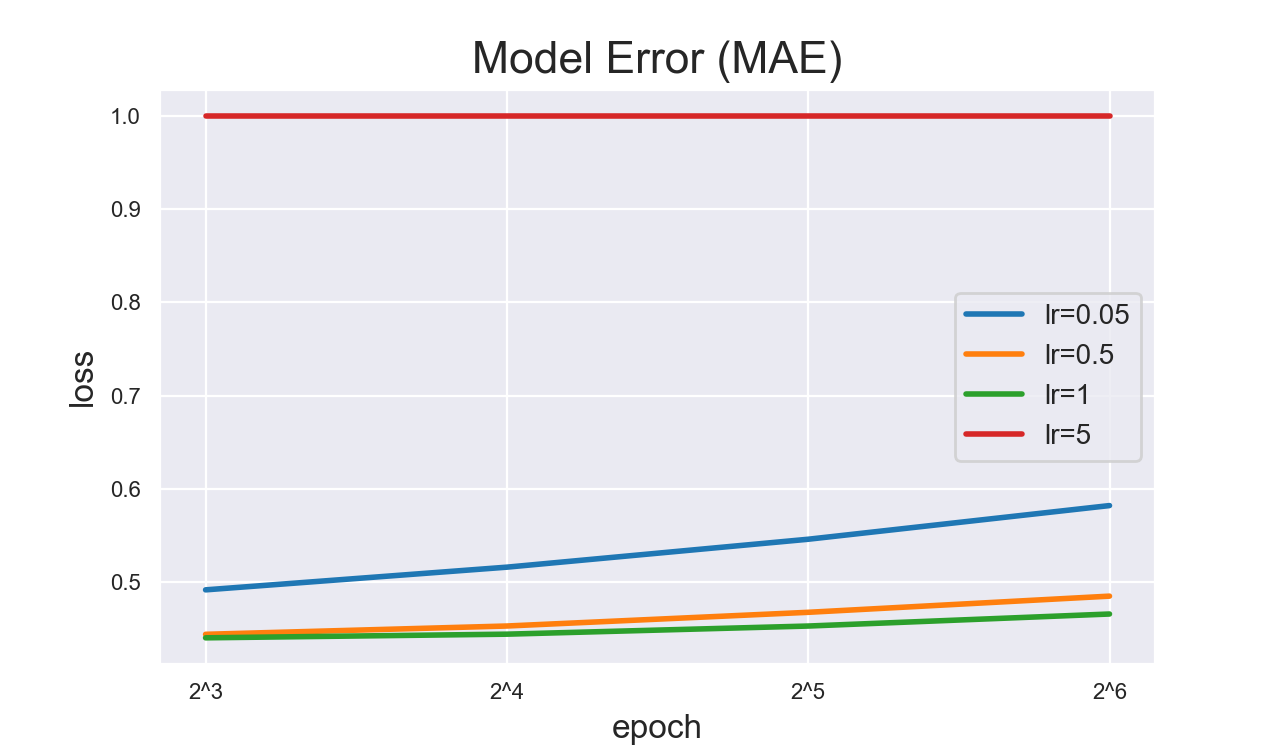
\includegraphics[width=0.90\textwidth]{./assets/MLP_MAE.png}
        \caption{不同超参数下，模型在测试集上的均方误差}
        \end{figure}

        经实验比较，我们选取\textbf{学习率为1}，\textbf{batch\_size为8}作为最优的超参数，
        此时模型在测试集上的\textbf{均方误差为0.4465}，\textbf{平均绝对误差为0.4404}，满足题目中MSE小于0.6的要求。

        最终模型在训练过程中的损失函数的变化曲线与每个epoch后模型在验证集上的损失函数变化曲线如图6所示。

        \begin{figure}[htbp]
        \centering
        \subfigure[训练集上的损失函数的变化曲线]{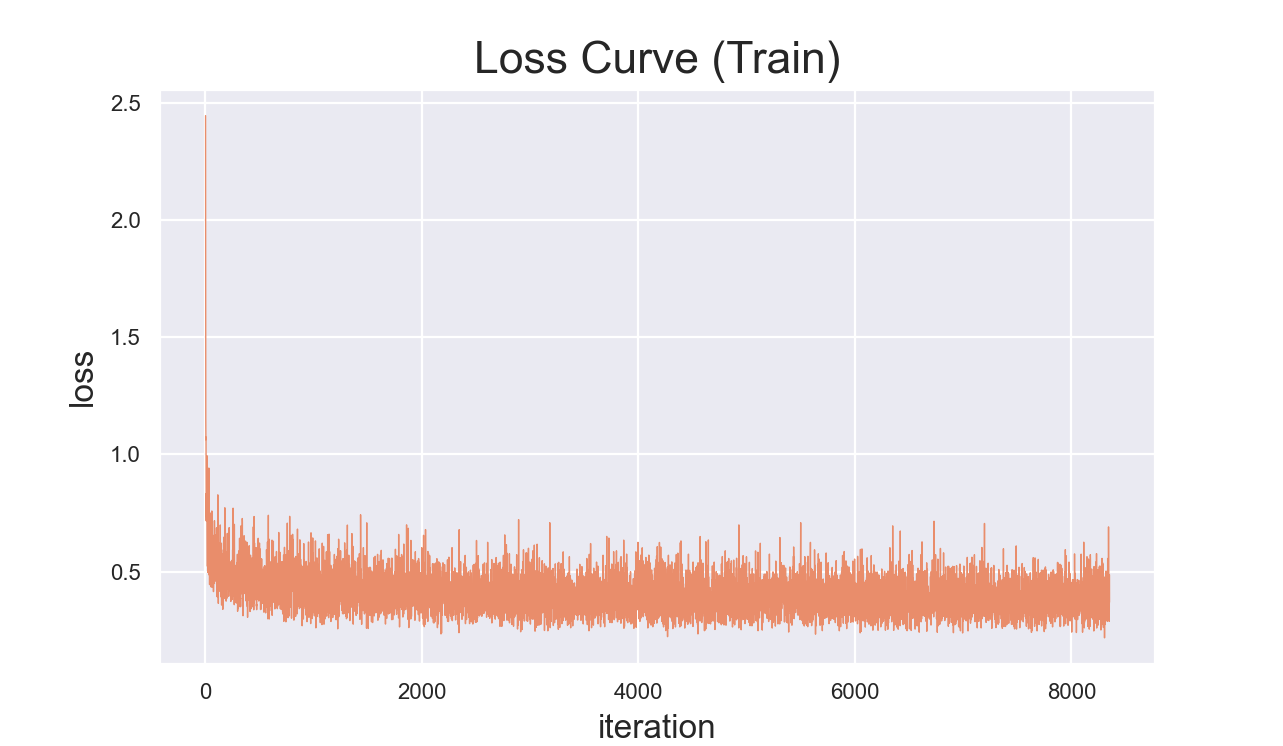
\includegraphics[width=0.48\textwidth]{./assets/MLP_final_train.png}}
        \subfigure[验证集上的损失函数的变化曲线]{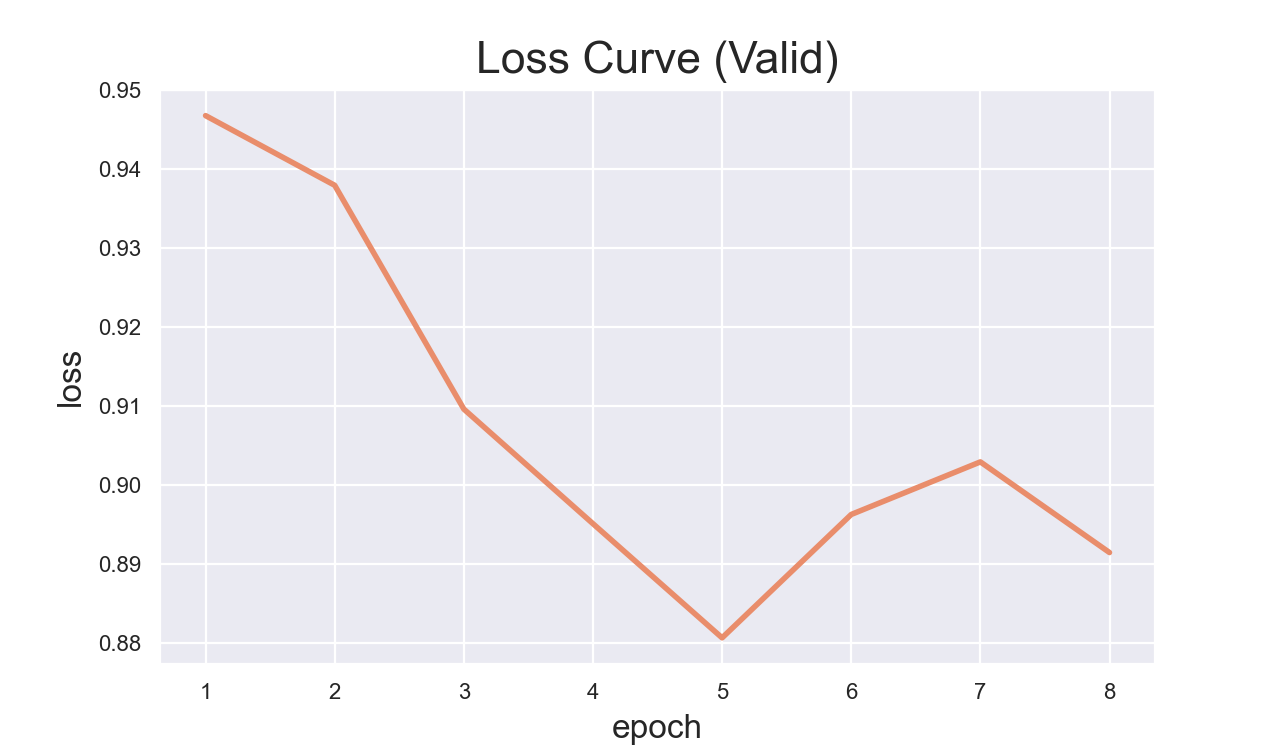
\includegraphics[width=0.48\textwidth]{./assets/MLP_final_valid.png}}
        \caption{最终模型的训练曲线}
        \end{figure}

        最终模型的缓存与相关的测试结果请参考./MLP中的相关文件。

\section{Convolutional Neural Network}

    \stepcounter{subsection}

    \stepcounter{subsection}

    \stepcounter{subsection}

    \subsection{Task Description}

    运行环境为：Windows 10 22H2，Python 3.9.18，PyTorch 1.12.1。

    \textbf{[Task A]}

    You are required to use the architecture of ResNet-18 to train a new model from scratch on the training set and then evaluate on the given test set.

    \textbf{[Task B]}

    Design and implement your own convolutional neural networks (CNNs) to train a new model from scratch on the training set and then evaluate on the given test set.

    \subsubsection{Train a model A for Task A, evaluate its AUC on test set, and report training and test curves.}

        model A是ResNet\_18模型。 \endnote{K. He, X. Zhang, S. Ren, and J. Sun. Deep residual learning for image recognition. In CVPR, 2016.}
        在Task A中，我们将直接调用torchvision库的相关接口，使用该模型完成图像分类任务。

        固定随机数种子为42，取batch\_size为256，num\_epoch为10，学习率为0.0001。
        运行./CNN/main.py。取Smoothing=0.6，使用TensorBoard，我们绘制出模型在训练集、验证集上的AUC值、损失函数值的变化情况如图7、图8所示。

        观察曲线可知：在训练集上，AUC值曲线的上升情况与损失函数值曲线的下降情况均保持稳定，说明模型学习进程正常；
        在验证集上AUC值曲线先上升到最大值，然后逐渐下降，说明模型已经收敛到拟合状态较好的参数位置。

        在验证集上，模型在epoch为6时取到最大的AUC值，为\textbf{0.7136}，此时模型的损失函数值为0.3004。

        \begin{figure}[htbp]
        \centering
        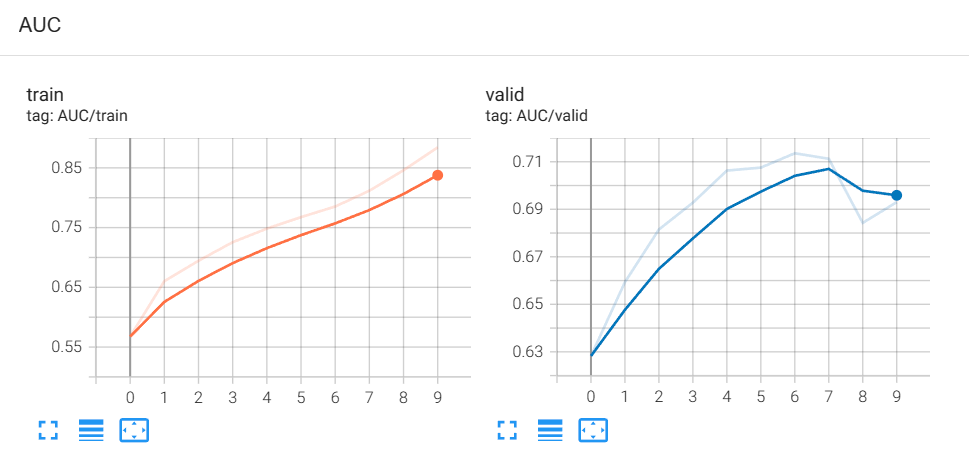
\includegraphics[width=0.96\textwidth]{./assets/resnet18_AUC.png}
        \caption{model A在训练集、验证集上的AUC值变化情况}
        \end{figure}

        \begin{figure}[htbp]
        \centering
        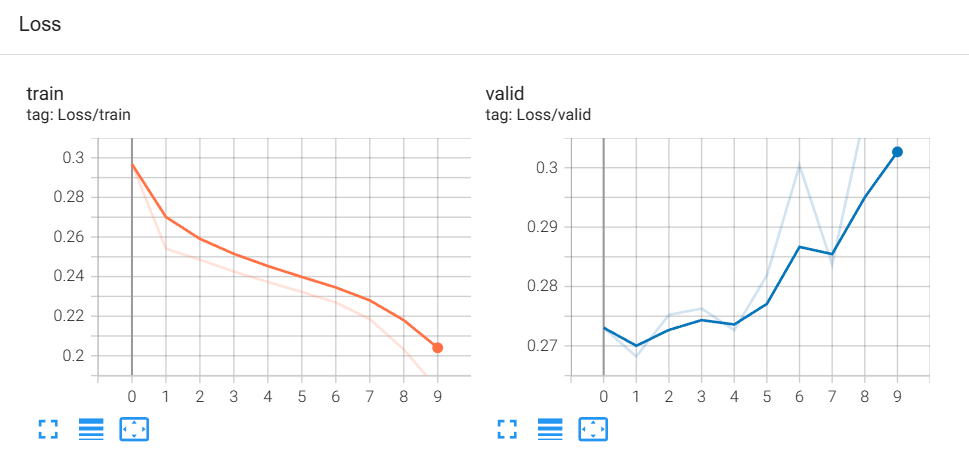
\includegraphics[width=0.96\textwidth]{./assets/resnet18_Loss.png}
        \caption{model A在训练集、验证集上的损失函数值变化情况}
        \end{figure}

        \subsubsection{Leverage a proper neural network visualization toolkit to visualize conv features or saliency maps of model A.}

        我们\textbf{实现了可视化conv features和saliency maps的相关代码}，详请参见./CNN/visualize.py文件。

        在实现过程中，我参考了以下Blog和Repository的内容：

        \begin{enumerate}
            \item https://github.com/utkuozbulak/pytorch-cnn-visualizations
            \item https://zhuanlan.zhihu.com/p/663895749
            \item https://blog.csdn.net/u011668104/article/details/108288694
            \item https://github.com/conda-forge/grad-cam-feedstock
        \end{enumerate}

        绘制得到的\textbf{con features}如图9所示。

        可以看出，各卷积核处理后的图像信息并不一致。
        具体而言，浅层的卷积核倾向于提取图像细节的、局部的信息，形式也更为具体，能够被人类所理解。
        而深层的卷积核则更注重宏观的、整体的信息，其形式较为抽象，和人类的直接认知有一定差别。

        \begin{figure}[htbp]
        \centering
        \includegraphics[width=0.96\textwidth]{./assets/resnet18_conv_features.png}
        \caption{Conv Features of model A (ResNet\_18)}
        \end{figure}

        绘制得到的\textbf{saliency maps}如图10所示。

        图中的亮点代表了高显著性的位置。
        可以看出，在我们选取的9张样例输入图片中，肺部、支气管等部位的显著性明显较高。
        这意味着，经训练的模型认为这些部位的图像特征对病种分类任务而言较为重要，
        这一点同我们人类的认知是一致的，从结果层面印证了卷积神经网络算法的有效性和合理性。

        \begin{figure}[htbp]
        \centering
        \subfigure{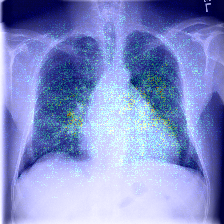
\includegraphics[width=0.30\textwidth]{./assets/resnet18_saliency_map_1.png}}
        \subfigure{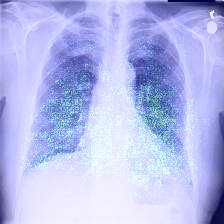
\includegraphics[width=0.30\textwidth]{./assets/resnet18_saliency_map_2.png}}
        \subfigure{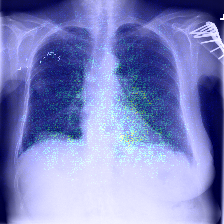
\includegraphics[width=0.30\textwidth]{./assets/resnet18_saliency_map_3.png}}
        \quad
        \subfigure{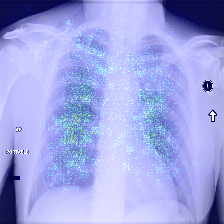
\includegraphics[width=0.30\textwidth]{./assets/resnet18_saliency_map_4.png}}
        \subfigure{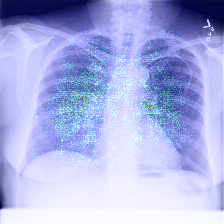
\includegraphics[width=0.30\textwidth]{./assets/resnet18_saliency_map_5.png}}
        \subfigure{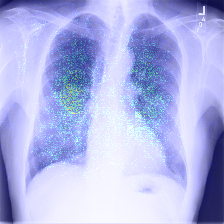
\includegraphics[width=0.30\textwidth]{./assets/resnet18_saliency_map_6.png}}
        \quad
        \subfigure{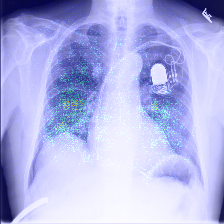
\includegraphics[width=0.30\textwidth]{./assets/resnet18_saliency_map_7.png}}
        \subfigure{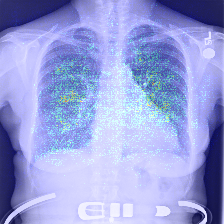
\includegraphics[width=0.30\textwidth]{./assets/resnet18_saliency_map_8.png}}
        \subfigure{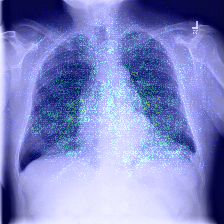
\includegraphics[width=0.30\textwidth]{./assets/resnet18_saliency_map_9.png}}
        \caption{模型在测试集上的预测结果}
        \end{figure}

    \subsubsection{Train a model B for Task B, evaluate its AUC on test set, and report training and test curves.}

        参考torchvision中提供的ResNet\_18模型的源代码和ConvNeXt模型的设计思想，结合在实验中获取的经验，我们完成了model B的设计。 \endnote{Z. Liu, H. Mao, C. Wu, C. Feichtenhofer, T. Darrell, and S. Xie. A convnet for the 2020s. In CVPR, 2022.}

        模型结构如图11所示，我们将该模型命名为MyConvNeXt\_v1。

        \begin{figure}[htbp]
        \centering
        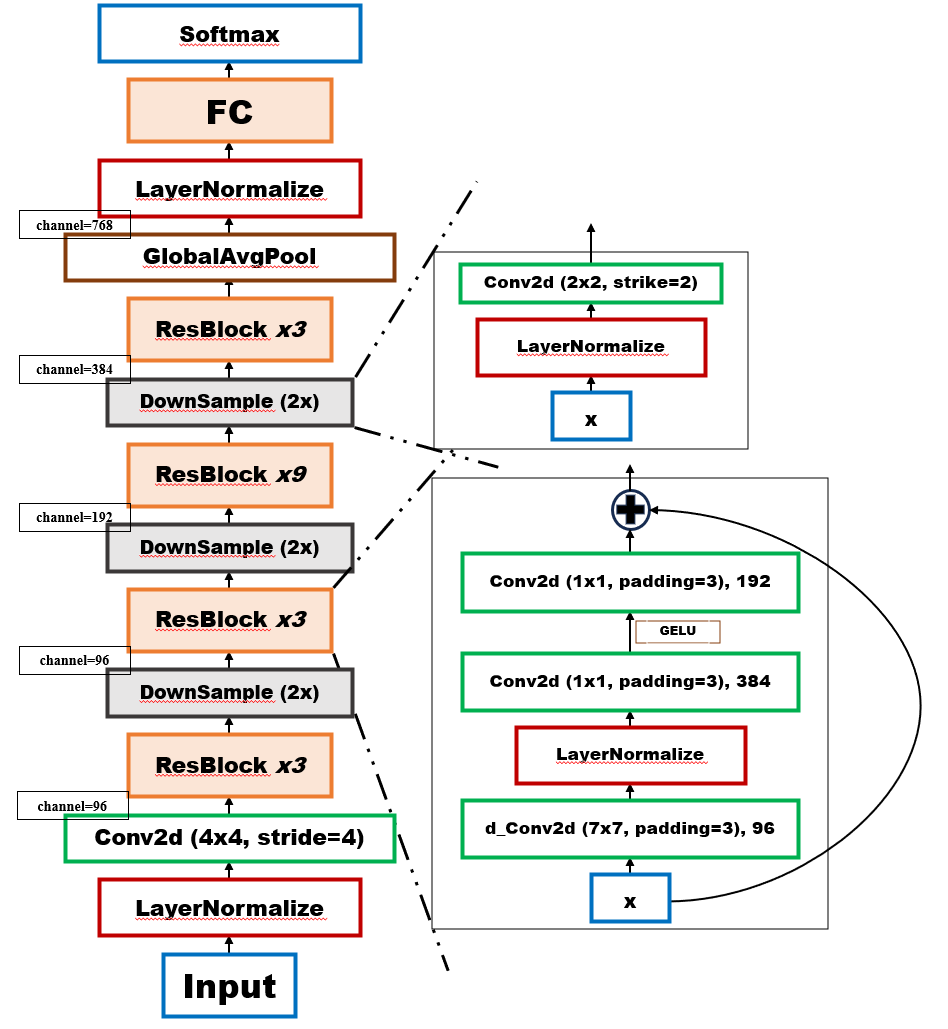
\includegraphics[width=1\textwidth]{./assets/MyConvNeXt.png}
        \caption{MyConvNeXt\_v1结构示意图}
        \end{figure}

        具体而言，依据ConvNeXt模型的改进思路，相较于ResNet\_18模型，MyConvNeXt\_v1模型的主要修改如下：

        \begin{enumerate}
            \item 将激活函数ReLU()更改为GeLU()。
            \item 将Batch\_Normalization更改为Layer\_Normalization。
            \item 在重新设计的残差子模块ResBlock中，使用了7x7大小的深度分离卷积核，后接两个1x1的卷积核以构建Inverted Bottleneck结构。如此，在提高模块拟合能力的同时，也降低了计算量。
            \item 调整了各stage中残差子模块的数量。
        \end{enumerate}

        考虑到本问题中分类数较少，我们适当减少了MyConvNeXt\_v1模型中的中间通道数大小，并降低了残差子模块中卷积核的大小，希望能够提升模型的效率。

        将MyConvNeXt\_v1模型中的中间通道数大小降低$33\%$，并改用5x5大小的卷积核，得到了模型MyConvNeXt\_v2。

        将MyConvNeXt\_v1模型中的中间通道数大小降低$50\%$，并改用5x5大小的卷积核，得到了模型MyConvNeXt\_v3。

        另外，我们希望能够将DenseNet中密集连接的思想融入模型中，以进一步提升模型的效果。 \endnote{G. Huang, Z. Liu, L. van der Maaten, and K. Q. Weinberger. Densely connected convolutional networks. In CVPR, 2017.}
        将MyConvNeXt\_v1模型中的每一个stage内部的子模块修改为密集连接方式，并适当调整中间通道数大小和stage中残差子模块的数量，
        得到了模型MyDenseNet。

        各个模型的代码实现详请参见./CNN/models.py中的有关内容。

        固定随机数种子为42，取学习率为0.0001，在数据集上训练模型。

        取Smoothing=0.6，各模型在训练集、验证集上的AUC值、损失函数值的变化情况如图12所示。

        可以看出，在10个epoch左右，各个模型均已收敛到了效果较好的拟合位置。

        \begin{figure}[htbp]
        \centering
        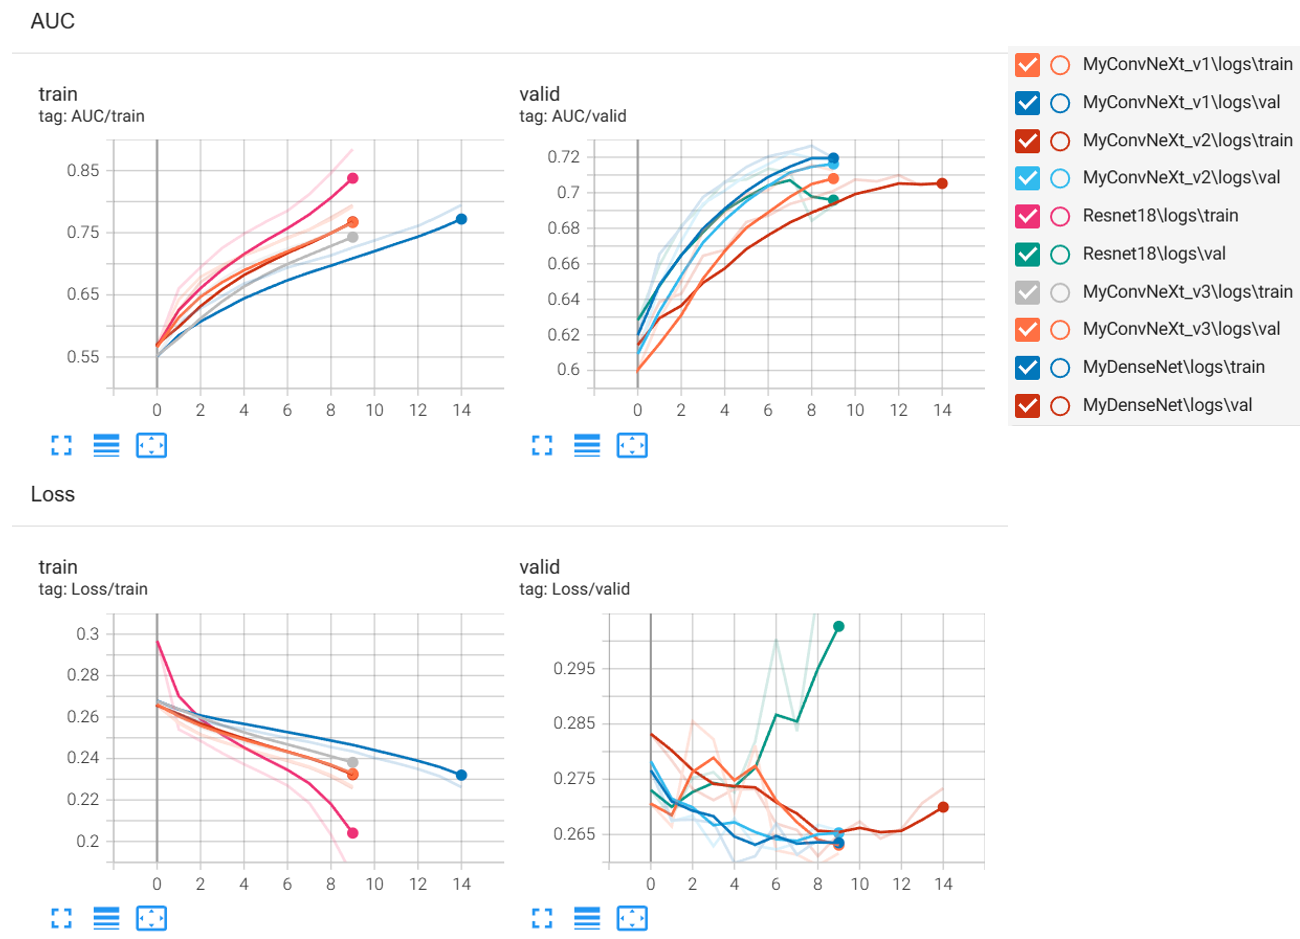
\includegraphics[width=1\textwidth]{./assets/MyNet.png}
        \caption{各模型在训练集、验证集上的AUC值、损失函数值的变化情况}
        \end{figure}

        我们以验证集上的最大AUC值作为评价模型效果的标准（val loss），各模型的实验结果如表1所示。

        从实验结果中可以看出，三个类ConvNeXt模型的效果较好，均优于ResNet18模型。
        \textbf{其中MyConvNeXt\_v1模型效果最好，其AUC值较ResNet18模型高0.0128，性能提升了1.803\%。}

        注意到，随着中间层通道数的减少和卷积核的缩小，三个版本的MyConvNeXt模型的性能有所损失，
        说明较多的中间层通道数和大卷积核确实有利于模型捕捉图像特征。
        另外，三个版本的MyConvNeXt模型的训练耗时也逐步减少，其中MyConvNeXt\_v3模型在耗时低于ResNet18模型的前提下，取得了更好的效果。
        这说明类ConvNeXt模型的结构设计较传统ResNet模型更好，具有更高的参数利用效率。

        \begin{table}[htbp]
        \caption{各模型的实验结果}
        \centering
        \begin{tabular}{cccccc}
            \toprule
            model           & val AUC          & val loss & train AUC & train loss & time cost  \\
            \midrule
            ResNet18        & \textbf{0.7136}  & 0.2599   & 0.8843    & 0.1833     & 4min/epoch \\
            MyConvNeXt\_v1  & \textbf{0.7264}  & 0.2599   & 0.7920    & 0.2265     & 9min/epoch \\
            MyConvNeXt\_v2  & \textbf{0.7223}  & 0.2623   & 0.7945    & 0.2257     & 5min/epoch \\
            MyConvNeXt\_v3  & \textbf{0.7155}  & 0.2594   & 0.7641    & 0.2337     & 3min/epoch \\
            MyDenseNet      & 0.7099           & 0.2611   & 0.7262    & 0.2435     & 6min/epoch
        \end{tabular}
        \end{table}

    \subsubsection{Use training techniques, including but not limited to data augmentation and learning rate strategies, either sourced from existing materials or proposed by yourself, to improve the performance of your model B and give a detailed ablation study in your report.}

        在最后，我们希望使用一些数据增强方法和学习率调整策略，来进一步提升模型的性能。

        根据表1结果，MyConvNeXt\_v3模型在具有较高性能的同时，训练速度较快。
        因此，出于实验效率考虑，我们在本节中使用MyConvNeXt\_v3模型作为基础实验模型。

        我们设计了三种数据增强方法，分别是：

        \begin{enumerate}
            \item 以0.5的概率对图像作随机水平翻转。
            \item 以0.5的概率对图像作随机擦除。
            \item 对图像作高斯模糊处理。
        \end{enumerate}

        三种方法的代码实现参见./CNN/data.py中的data\_transforms字典。

        我们认为，在医学图像处理问题中，肺部处在正确的位置上是一个重要的信息，故采用垂直反转、旋转等方法的效果不会太好。
        因此我们并未采取随机垂直反转，随机旋转等数据增强方式。

        固定随机数种子为42，取学习率为0.0001，采用不同的数据增强方法，在数据集上训练模型。

        取Smoothing=0.6，各模型在训练集、验证集上的AUC值、损失函数值的变化情况如图13所示。

        \begin{figure}[htbp]
        \centering
        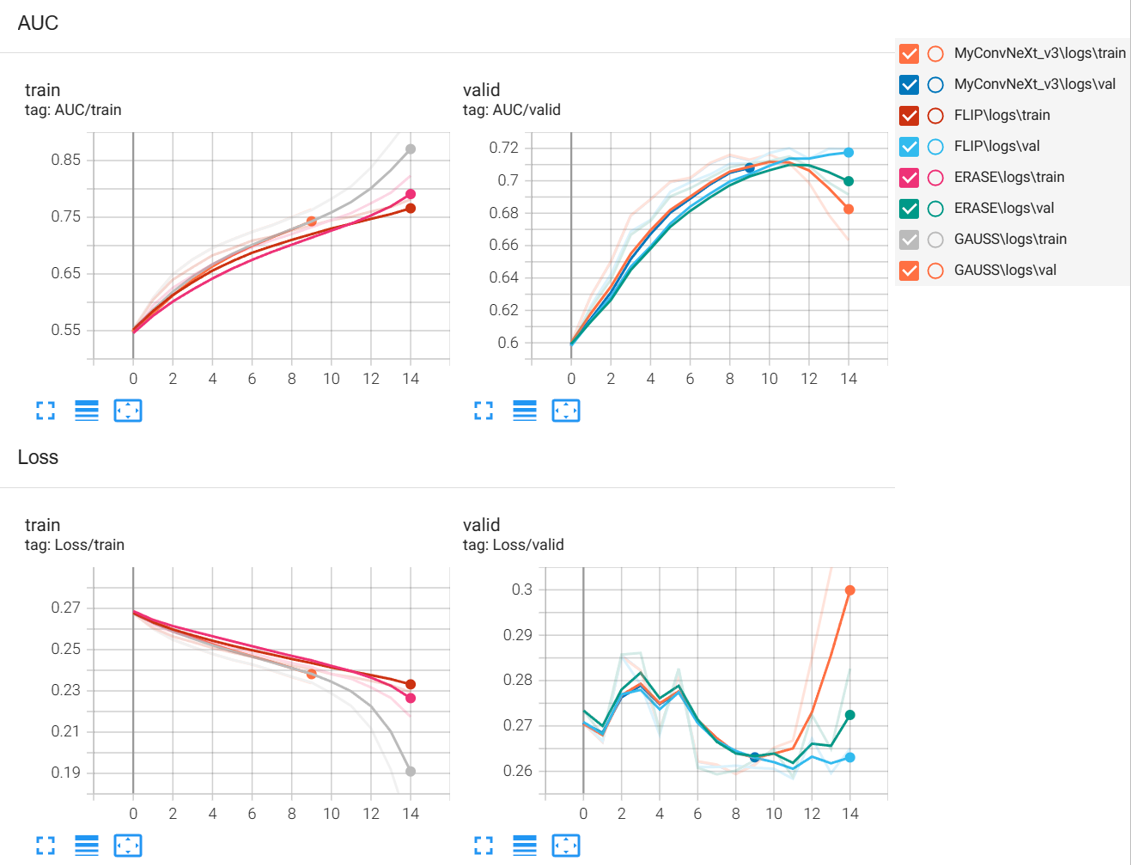
\includegraphics[width=1\textwidth]{./assets/Data_Augmentation.png}
        \caption{使用数据增强方法后，模型在训练过程中的性能变化情况}
        \end{figure}

        从图中可以看出，在采用了数据增强方法后，模型的收敛速度下降，同时后期的过拟合程度也有所减轻（高斯模糊处理除外）。
        这是因为随机水平翻转和随机擦除方法等价于强化了模型的正则项。
        我们猜测，高斯模糊处理没能够减轻模型过拟合程度的原因，可能是模糊处理将降低模型“作弊”的难度。

        实验结果如表2所示。可见\textbf{随机水平翻转}和\textbf{高斯模糊处理}能够提升模型的性能。

        \begin{table}[htbp]
        \caption{各数据增强方法的实验结果}
        \centering
        \begin{tabular}{ccccc}
            \toprule
            Augmentation   & val AUC          & val loss \\
            \midrule
            Default        & \textbf{0.7155}  & 0.2594   \\
            HorizontalFlip & \textbf{0.7202}  & 0.2584   \\
            Erase          & 0.7149           & 0.2593   \\
            GaussianBlur   & \textbf{0.7163}  & 0.2594
        \end{tabular}
        \end{table}

        我们设计了四种学习率调整策略，分别是：
        \begin{enumerate}
            \item 线性降低策略：学习率将线性地降低至2e-5。
            \item 指数降低策略：每个epoch后，学习率将乘以0.9。
            \item 余弦退火策略：学习率将呈余弦函数变化，共1.5个周期，最小值2e-5。
            \item 余弦退火策略：学习率将呈余弦函数变化，共0.5个周期，最小值2e-5。
        \end{enumerate}

        四种策略的代码实现参见./CNN/main.py中注释标记的部分。

        固定随机数种子为42，取初始学习率为0.0001，采用学习率调整策略，在数据集上训练模型。

        取Smoothing=0.6，各模型在训练集、验证集上的AUC值、损失函数值的变化情况如图14所示。

        \begin{figure}[htbp]
        \centering
        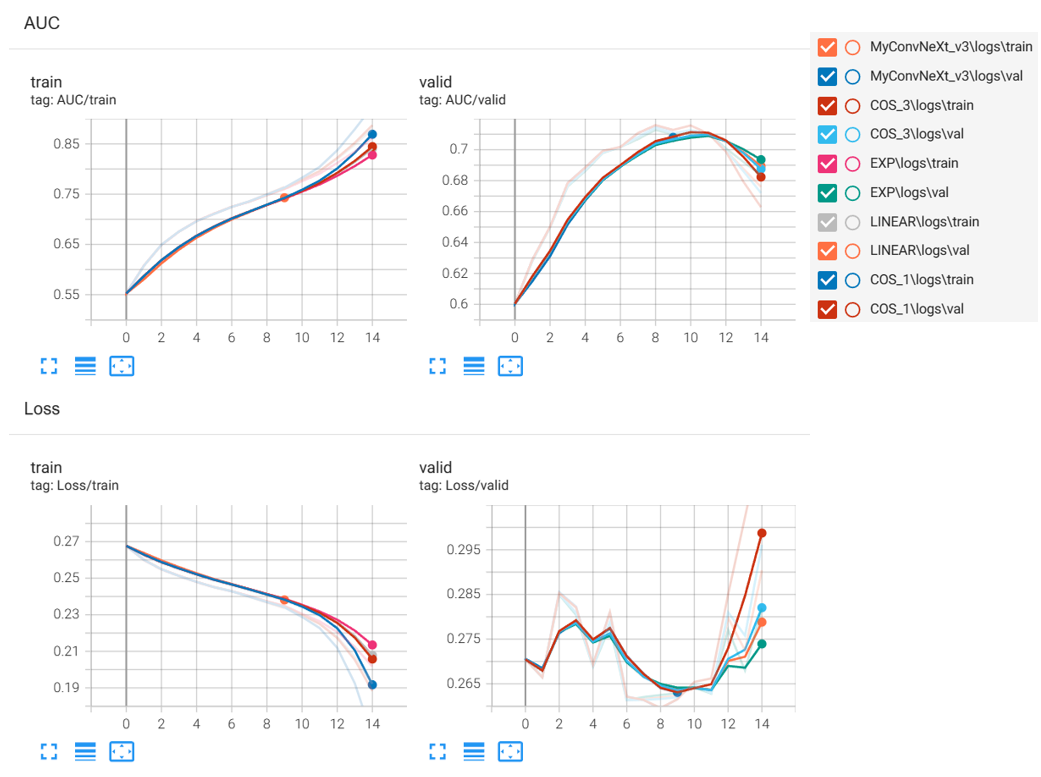
\includegraphics[width=1\textwidth]{./assets/LR_Strategies.png}
        \caption{使用学习率策略方法后，模型在训练过程中的性能变化情况}
        \end{figure}

        从图中可以看出，在采用了学习率调整策略后，模型在前期的收敛速度几乎不受影响，而后期的收敛速度明显降低，
        因此更容易收敛到较为合适的拟合位置。

        实验结果如表3所示。可见\textbf{0.5个周期的余弦退火策略}能够提升模型的性能。

        \begin{table}[htbp]
        \caption{各学习率调整策略的实验结果}
        \centering
        \begin{tabular}{ccccc}
            \toprule
            Augmentation             & val AUC          & val loss \\
            \midrule
            Default                  & \textbf{0.7155}  & 0.2594   \\
            LinearLR                 & 0.7138           & 0.2613   \\
            ExponentialLR            & 0.7128           & 0.2614   \\
            CosineAnnealingLR(T=1.5) & 0.7141           & 0.2613   \\
            CosineAnnealingLR(T=0.5) & \textbf{0.7159}  & 0.2596
        \end{tabular}
        \end{table}

        最终，我们在MyConvNeXt\_v1模型的基础上，结合随机水平翻转、高斯模糊处理的数据增强方法和0.5个周期的余弦学习率退火策略，
        改进得到了效果最好的model B。

        取Smoothing=0.6，model A和model B在训练集、验证集上的AUC值、损失函数值的变化情况如图15所示。

        \begin{figure}[htbp]
        \centering
        \includegraphics[width=0.84\textwidth]{./assets/final.png}
        \caption{model A/B在训练过程中的性能变化情况}
        \end{figure}

        从图中可以看出，model B的收敛速度更慢，但其在验证集上的最大AUC值和最低loss均显著低于model A。

        实验结果如表4所示。

        \begin{table}[htbp]
        \caption{各学习率调整策略的实验结果}
        \centering
        \begin{tabular}{ccccc}
            \toprule
            model   & val AUC          & val loss \\
            \midrule
            model A & \textbf{0.7136}  & 0.2594   \\
            model B & \textbf{0.7276}  & 0.2613
        \end{tabular}
        \end{table}

        结论：\textbf{model B性能较高，AUC值较model A模型高0.0140，性能提升了1.962\%}。

        最终模型的缓存文件位于./CNN/checkpoints中。

\theendnotes

\end{document}
